%==============================================================================
%  LAB REPORT 2 — Binary Representation of Numbers Using LEDs
%  Compile with pdfLaTeX (works out of the box on Overleaf).
%
%  >>> PASTE YOUR GOOGLE DRIVE LINKS IN THE MACROS MARKED "EDIT ME" BELOW <<<
%==============================================================================
\documentclass[10pt,a4paper]{article}

%---------------------------------------- page geometry
\usepackage[a4paper,top=2.2cm,bottom=2.0cm,left=2.1cm,right=2.1cm,
            headsep=13pt,footskip=22pt]{geometry}

%---------------------------------------- encoding & fonts
\usepackage[T1]{fontenc}
\usepackage[utf8]{inputenc}
\usepackage{newtxtext,newtxmath}     % Times-like professional text + math
\usepackage[scaled=0.86]{beramono}   % clean monospace for code
\usepackage{microtype}

%---------------------------------------- graphics, colour, boxes
\usepackage{graphicx}
\usepackage[dvipsnames,table]{xcolor}
\usepackage{tikz}
\usepackage{circuitikz}
\usepackage[most]{tcolorbox}
\usepackage{booktabs}
\usepackage{array}
\usepackage{tabularx}
\usepackage{enumitem}
\usepackage{listings}
\usepackage{fancyhdr}
\usepackage{titlesec}
\usepackage{caption}
\usepackage{float}
\usepackage{needspace}
\usetikzlibrary{arrows.meta,positioning,calc,shadows.blur}
\ctikzset{bipoles/length=0.62cm}   % compact component symbols

%---------------------------------------- hyperlinks (load late)
\usepackage[hidelinks]{hyperref}
\usepackage{url}
% print a URL stored in a macro, safely (handles _ ~ % etc.)
\newcommand{\showurl}[1]{\expandafter\url\expandafter{#1}}

%==============================================================================
%  Student details
%==============================================================================
\newcommand{\studentname}{Chavan Atharva Sunil}
\newcommand{\rollnumber}{240003021}
\newcommand{\coursecode}{AA303 --- IoT for Space Applications}
\newcommand{\expdate}{13 August 2026}   % <-- CHECK THIS DATE

%  Google Drive folder holding the demonstration videos and the source code
\urldef{\drivefolder}\url{https://drive.google.com/drive/folders/1cdR2mrryf5j0LEnQgIgYEAs-zB0Qj0jO?usp=sharing}

%==============================================================================
%  Colour palette
%==============================================================================
\definecolor{ink}{HTML}{1B2733}      % body text / headings
\definecolor{accent}{HTML}{0B5FA5}   % primary blue
\definecolor{accentlt}{HTML}{E8F1FA} % pale blue fill
\definecolor{amber}{HTML}{C8791A}    % LED amber
\definecolor{amberlt}{HTML}{FDF3E3}
\definecolor{rule}{HTML}{C9D4DE}
\definecolor{soft}{HTML}{F5F7F9}
\definecolor{codebg}{HTML}{F7F9FB}
\definecolor{cmnt}{HTML}{6C8090}
\definecolor{kw}{HTML}{0B5FA5}
\definecolor{str}{HTML}{1C7C54}
\definecolor{num}{HTML}{9B2D5E}

\color{ink}

%==============================================================================
%  Headings
%==============================================================================
\titleformat{\section}
  {\normalfont\large\bfseries\color{accent}}
  {\raisebox{0pt}{\colorbox{accent}{\color{white}\bfseries\;\thesection\;}}}
  {0.7em}{}[\vspace{2pt}{\color{rule}\titlerule[0.8pt]}]
\titlespacing*{\section}{0pt}{14pt}{8pt}

\titleformat{\subsection}
  {\normalfont\normalsize\bfseries\color{ink}}{\thesubsection}{0.6em}{}
\titlespacing*{\subsection}{0pt}{11pt}{4pt}

\titleformat{\subsubsection}
  {\normalfont\small\bfseries\color{accent}}{}{0em}{}
\titlespacing*{\subsubsection}{0pt}{9pt}{2pt}

%==============================================================================
%  Header / footer
%==============================================================================
\pagestyle{fancy}
\fancyhf{}
\renewcommand{\headrulewidth}{0.4pt}
\renewcommand{\footrulewidth}{0pt}
\fancyhead[L]{\footnotesize\color{cmnt}\textsc{Lab Report 2} \,\textbar\, Binary Representation Using LEDs}
\fancyhead[R]{\footnotesize\color{cmnt}\studentname\ \,\textbar\, \rollnumber}
\fancyfoot[C]{\footnotesize\color{cmnt}\thepage}

%==============================================================================
%  Captions & lists
%==============================================================================
\captionsetup{font=small,labelfont={bf,color=accent},skip=6pt}
\setlist[itemize]{leftmargin=1.35em,itemsep=2pt,topsep=3pt}
\setlist[enumerate]{leftmargin=1.6em,itemsep=2.5pt,topsep=3pt}
\renewcommand{\arraystretch}{1.18}

%==============================================================================
%  Custom boxes
%==============================================================================
\newtcolorbox{keybox}[1][]{
  enhanced, breakable, colback=accentlt, colframe=accent,
  boxrule=0pt, leftrule=3pt, arc=2pt, left=10pt, right=10pt, top=8pt, bottom=8pt,
  fontupper=\normalsize, #1}

\newtcolorbox{notebox}[1][]{
  enhanced, breakable, colback=amberlt, colframe=amber,
  boxrule=0pt, leftrule=3pt, arc=2pt, left=10pt, right=10pt, top=7pt, bottom=7pt,
  fontupper=\small, #1}

\newtcolorbox{titledbox}[2][]{
  enhanced, breakable, colback=white, colframe=rule, boxrule=0.6pt, arc=3pt,
  left=10pt, right=10pt, top=8pt, bottom=8pt,
  title={\bfseries\small #2}, coltitle=white, colbacktitle=accent,
  attach boxed title to top left={xshift=8pt,yshift=-8pt},
  boxed title style={boxrule=0pt,arc=2pt,left=6pt,right=6pt,top=2pt,bottom=2pt},
  #1}

%==============================================================================
%  Code listing style
%==============================================================================
\lstdefinestyle{prostyle}{
  backgroundcolor=\color{codebg},
  basicstyle=\ttfamily\scriptsize\color{ink},
  keywordstyle=\color{kw}\bfseries,
  commentstyle=\color{cmnt}\itshape,
  stringstyle=\color{str},
  numberstyle=\ttfamily\tiny\color{cmnt},
  numbers=left, numbersep=9pt, xleftmargin=17pt, xrightmargin=2pt,
  frame=single, framesep=6pt, rulecolor=\color{rule},
  breaklines=true, showstringspaces=false, tabsize=2,
  columns=fullflexible, keepspaces=true,
  aboveskip=8pt, belowskip=6pt,
  emphstyle=\color{num}\bfseries
}
\lstset{style=prostyle}

%==============================================================================
%  Reusable schematic macro
%  \gpioschematic{Board name}{p1}{p2}{p3}{p4}
%==============================================================================
\newcommand{\gpioschematic}[5]{%
\begin{circuitikz}[scale=0.86, transform shape, every node/.style={font=\footnotesize}]
  % ---- controller body
  \draw[fill=accentlt, draw=accent, line width=0.9pt, rounded corners=4pt]
        (-3.3,-0.15) rectangle (-0.6,4.9);
  \node[text=accent, font=\small\bfseries] at (-1.95,4.35) {#1};
  \node[text=cmnt,   font=\scriptsize]     at (-1.95,3.95) {GPIO header};

  % ---- pin pads + LED branches
  \foreach \y/\pin/\led in {3.15/#2/1, 2.2/#3/2, 1.25/#4/3, 0.3/#5/4}{
     \draw[fill=white, draw=accent, line width=0.6pt]
           (-0.92,\y-0.14) rectangle (-0.6,\y+0.14);
     \node[anchor=east, font=\scriptsize\bfseries, text=accent]
           at (-1.02,\y) {\pin};
     \draw[line width=0.7pt, accent] (-0.6,\y) -- (0.6,\y);
     \draw[line width=0.7pt] (0.6,\y) to[leD, l=LED\,\led] (3.6,\y);
     \draw[line width=0.7pt] (3.6,\y) -- (5.0,\y);
     \fill (5.0,\y) circle (1.3pt);
  }
  % ---- common ground rail
  \draw[line width=1pt] (5.0,0.3) -- (5.0,3.15);
  \draw[line width=1pt] (5.0,0.3) -- (5.0,-0.45);
  \node[ground] at (5.0,-0.45) {};
  \node[anchor=west, font=\scriptsize\bfseries] at (5.15,-0.3) {GND};
  \node[anchor=north, font=\scriptsize, text=cmnt, align=center]
        at (1.4,-0.95) {common ground rail on the breadboard, returned to the board's GND pin};
\end{circuitikz}}

% \gpioschematiceight{board}{p1}..{p8}   (p1 = MSB, p8 = LSB)
\newcommand{\gpioschematiceight}[9]{%
\begin{circuitikz}[scale=0.84, transform shape, every node/.style={font=\footnotesize}]
  \draw[fill=accentlt, draw=accent, line width=0.9pt, rounded corners=4pt]
        (-3.5,-0.15) rectangle (-0.6,8.05);
  \node[text=accent, font=\small\bfseries] at (-2.05,7.5) {#1};
  \node[text=cmnt,   font=\scriptsize]     at (-2.05,7.1) {GPIO header};
  \foreach \y/\pin/\bit/\wt in {%
      6.3/#2/7/128, 5.4/#3/6/64, 4.5/#4/5/32, 3.6/#5/4/16,
      2.7/#6/3/8,   1.8/#7/2/4,  0.9/#8/1/2,  0.0/#9/0/1}{
     \draw[fill=white, draw=accent, line width=0.6pt]
           (-0.92,\y-0.14) rectangle (-0.6,\y+0.14);
     \node[anchor=east, font=\scriptsize\bfseries, text=accent] at (-1.02,\y) {\pin};
     \draw[line width=0.7pt, accent] (-0.6,\y) -- (0.6,\y);
     \draw[line width=0.7pt] (0.6,\y) to[leD, l=LED\,\bit] (3.6,\y);
     \draw[line width=0.7pt] (3.6,\y) -- (5.0,\y);
     \fill (5.0,\y) circle (1.3pt);
     \node[anchor=west, font=\scriptsize, text=amber] at (5.25,\y) {bit \bit\ ($\wt$)};}
  \draw[line width=1pt] (5.0,0.0) -- (5.0,6.3);
  \draw[line width=1pt] (5.0,0.0) -- (5.0,-0.75);
  \node[ground] at (5.0,-0.75) {};
  \node[anchor=west, font=\scriptsize\bfseries] at (5.15,-0.6) {GND};
  \node[anchor=north, font=\scriptsize, text=cmnt, align=center]
        at (1.6,-1.25) {common ground rail on the breadboard, returned to the board's GND pin};
\end{circuitikz}}

%==============================================================================
\begin{document}

%------------------------------------------------------------------ TITLE BLOCK
\thispagestyle{empty}
\begin{tikzpicture}[remember picture, overlay]
  \fill[accent] (current page.north west) rectangle
        ($(current page.north east)+(0,-7.15cm)$);
  \fill[amber] ($(current page.north west)+(0,-7.15cm)$) rectangle
        ($(current page.north east)+(0,-7.3cm)$);
\end{tikzpicture}

\vspace*{0.35cm}
{\color{white}
 \noindent{\footnotesize\textsc{\coursecode}}\\[2pt]
 \noindent{\Large\bfseries Experiment 2 \,\textbar\, Lab Report}\\[8pt]
 \noindent{\huge\bfseries Binary Representation of}\\[6pt]
 \noindent{\huge\bfseries Numbers Using LEDs}\\[10pt]
 \noindent{\small Displaying a decimal number on eight GPIO-driven LEDs (Raspberry Pi)}
}
\vspace{1.5cm}

\noindent
\begin{tabularx}{\textwidth}{@{}>{\bfseries\color{accent}}l X@{}}
\toprule
Submitted by  & \studentname \\
Roll Number   & \rollnumber \\
Date of Experiment & \expdate \\
Board Used    & Raspberry Pi (BOARD numbering) \\
\bottomrule
\end{tabularx}

\vspace{10pt}

%------------------------------------------------------------------ 1. AIM
\section{Aim}

\begin{keybox}
To represent a decimal number in \textbf{binary} form using eight LEDs driven from the
GPIO pins of a \textbf{Raspberry Pi}. The user enters a number in the range
$0$--$255$ at the terminal; the program converts it to its 8-bit binary equivalent and
lights one LED per set bit, so that the row of LEDs can be read directly as the binary
value of the number entered.
\end{keybox}

\subsection*{Objectives}
\begin{itemize}
  \item To configure eight GPIO pins of the Raspberry Pi as digital outputs and wire
        one LED to each.
  \item To read a decimal number from the user and convert it to a fixed-width 8-bit
        binary string in software.
  \item To map each bit of that string to its corresponding GPIO pin, so that the
        illuminated LEDs form the binary representation of the number.
  \item To verify the displayed pattern against the binary string printed on the
        console for several different inputs.
\end{itemize}

\subsection*{Brief Theory}
A GPIO pin configured as a digital output can be held at one of two levels: HIGH
($3.3\,\mathrm{V}$) or LOW ($0\,\mathrm{V}$). A single pin therefore carries exactly
one bit of information. Taking eight such pins together gives an 8-bit parallel output
port, capable of representing $2^{8} = 256$ distinct values, i.e.\ the integers
$0$ to $255$.

Each LED is assigned a \emph{place value} according to which bit it represents. The
leftmost LED carries $2^{7} = 128$ and the rightmost $2^{0} = 1$. Any number in range
can be written uniquely as a sum of these place values, and the corresponding pattern
of set bits is its binary representation. Displaying a number therefore reduces to
testing each of its eight bits in turn and driving the matching pin HIGH where the bit
is $1$ and LOW where it is $0$.

\begin{notebox}
\textbf{Note on current limiting.} The LEDs were connected \emph{directly} to the GPIO
pins, without series resistors, and the demonstration ran without damage. Each GPIO pin
can nevertheless source only a limited current (about $16\,\mathrm{mA}$ on the
Raspberry Pi), so for sustained use a series resistor of roughly $220\,\Omega$ per LED
--- giving $(3.3-2)/220 \approx 6\,\mathrm{mA}$ --- is the recommended practice.
\end{notebox}

%------------------------------------------------------------------ 2. MATERIALS
\Needspace{8\baselineskip}
\section{Materials Required}

\noindent
\begin{tabularx}{\textwidth}{@{}p{0.4cm} >{\raggedright\arraybackslash}p{5.2cm} c X@{}}
\toprule
\rowcolor{soft}
\multicolumn{1}{@{}l}{\textbf{\#}} & \textbf{Component} & \textbf{Qty.} & \textbf{Purpose in the setup} \\
\midrule
1 & Raspberry Pi (with SD card, OS installed) & 1 & Host board; drives the eight outputs \\
2 & Solderless breadboard                     & 1 & Mounting the LEDs and the ground rail \\
3 & LEDs (5\,mm, red)                         & 8 & One per bit of the 8-bit value \\
4 & Male--female jumper wires                 & 9--12 & GPIO header to breadboard connections \\
5 & USB power supply                          & 1 & Powering the Raspberry Pi \\
6 & Monitor, keyboard and mouse               & 1 & Entering the number at the terminal \\
\bottomrule
\end{tabularx}

%------------------------------------------------------------------ 3. METHODOLOGY
\section{Methodology}

Eight LEDs were placed in a row on the breadboard, each connected directly to its own
GPIO pin of the Raspberry Pi, with all cathodes tied to a common ground rail that was
returned to a GND pin of the board. The eight pins were configured as digital outputs
and initialised LOW, so that the display starts blank.

The program then loops: it reads a decimal number typed at the terminal, rejects
anything outside $0$--$255$, converts the value to an 8-bit binary string, and writes
the eight bits to the eight pins in order. The same string is printed back to the
console so that the illuminated row can be checked against the computed value.

\subsection{GPIO connections}

\vspace{2pt}
\noindent
\begin{minipage}[t]{0.48\textwidth}
\vspace{0pt}
\begin{tabularx}{\linewidth}{@{}l l X@{}}
\toprule
\rowcolor{soft}
\textbf{Bit} & \textbf{Place value} & \textbf{Raspberry Pi pin} \\
\midrule
bit 7 & 128 & Pin 40 \\
bit 6 & 64  & Pin 38 \\
bit 5 & 32  & Pin 36 \\
bit 4 & 16  & Pin 35 \\
bit 3 & 8   & Pin 33 \\
bit 2 & 4   & Pin 32 \\
bit 1 & 2   & Pin 31 \\
bit 0 & 1   & Pin 29 \\
\midrule
All cathodes & --- & GND \\
\bottomrule
\end{tabularx}
\end{minipage}\hfill
\begin{minipage}[t]{0.49\textwidth}
\vspace{0pt}
\begin{titledbox}{Numbering used here}
\raggedright
The program uses \textbf{BOARD} numbering (\texttt{GPIO.setmode(GPIO.BOARD)}), so the
numbers in the table are the \emph{physical} positions on the 40-pin header rather than
the Broadcom channel numbers. The most significant bit is wired at one end of the row
so that the LEDs read left-to-right in the same order as the binary string printed on
the console, which makes checking the output immediate.
\end{titledbox}
\end{minipage}

\begin{figure}[htb]
\centering
\gpioschematiceight{Raspberry Pi}{Pin 40}{Pin 38}{Pin 36}{Pin 35}{Pin 33}{Pin 32}{Pin 31}{Pin 29}
\caption{Circuit schematic. Eight LEDs are driven directly from eight GPIO pins, one
per bit, with all cathodes returned to the common ground rail on the breadboard.}
\label{fig:schematic}
\end{figure}

\subsection{Principle of operation}

A number is displayed by testing its bits one at a time and writing the result to the
matching pin, so the pattern of lit LEDs \emph{is} the binary representation of the
number. For example, $200 = 128 + 64 + 8$, giving the bit pattern \texttt{11001000}:

\begin{figure}[H]
\centering
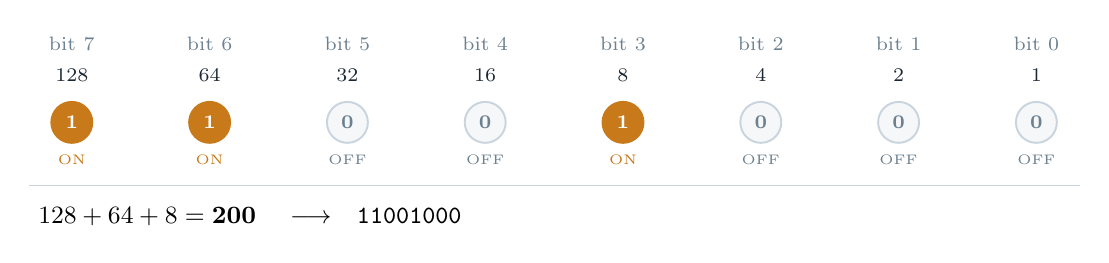
\begin{tikzpicture}[x=1cm, y=1cm]
  \foreach \i/\wt/\b in {0/128/1, 1/64/1, 2/32/0, 3/16/0, 4/8/1, 5/4/0, 6/2/0, 7/1/0}{
    \pgfmathsetmacro{\cx}{\i*1.75}
    \node[font=\scriptsize, text=cmnt] at (\cx,1.75) {bit \the\numexpr7-\i\relax};
    \node[font=\scriptsize\bfseries, text=ink] at (\cx,1.35) {$\wt$};
    \ifnum\b=1
      \fill[amber] (\cx,0.75) circle (0.26);
      \draw[amber, line width=0.7pt] (\cx,0.75) circle (0.26);
      \node[font=\scriptsize\bfseries, text=white] at (\cx,0.75) {1};
      \node[font=\tiny, text=amber] at (\cx,0.28) {ON};
    \else
      \fill[soft] (\cx,0.75) circle (0.26);
      \draw[rule, line width=0.7pt] (\cx,0.75) circle (0.26);
      \node[font=\scriptsize\bfseries, text=cmnt] at (\cx,0.75) {0};
      \node[font=\tiny, text=cmnt] at (\cx,0.28) {OFF};
    \fi}
  \draw[rule, line width=0.6pt] (-0.55,-0.05) -- (12.8,-0.05);
  \node[font=\small, anchor=west] at (-0.55,-0.45)
       {$128 + 64 + 8 = \mathbf{200}$ \quad$\longrightarrow$\quad \texttt{11001000}};
\end{tikzpicture}
\caption{Place values of the eight LEDs and the pattern displayed for the input $200$.}
\label{fig:bits}
\end{figure}

\subsection{Procedure}
\begin{enumerate}
  \item Eight LEDs were placed in a row on the breadboard with all cathodes on the
        common ground rail, which was returned to a GND pin of the Raspberry Pi.
  \item Each anode was wired to its own GPIO pin in the order given in the table above,
        the most significant bit first. The wiring was checked with the board powered off.
  \item The eight pins were configured as digital outputs and initialised LOW, leaving
        the display blank.
  \item The program was executed on the Raspberry Pi; it prompts for a decimal number
        at the terminal.
  \item The entered number was validated against the range $0$--$255$ and converted to
        an 8-bit binary string, zero-padded on the left so that it always has exactly
        eight digits.
  \item Each bit was written to its corresponding GPIO pin, lighting the LEDs that
        correspond to the set bits, and the binary string was printed to the console.
  \item Steps 4--6 were repeated for several different inputs and the illuminated
        pattern was compared against the printed string each time.
\end{enumerate}

\Needspace{12\baselineskip}
\subsection{Code (Python, Raspberry Pi)}

\begin{lstlisting}[language=Python, caption={Displaying a decimal number on eight LEDs as 8-bit binary.}, label={lst:rpi}]
import RPi.GPIO as GPIO

# Physical (BOARD) pin numbers, most significant bit first
LED_PINS = [40, 38, 36, 35, 33, 32, 31, 29]

GPIO.setmode(GPIO.BOARD)
GPIO.setwarnings(False)
for pin in LED_PINS:
    GPIO.setup(pin, GPIO.OUT, initial=GPIO.LOW)

try:
    while True:
        number = int(input("Enter a number (0-255): "))
        if not 0 <= number <= 255:
            print("Out of range - please enter a value from 0 to 255.")
            continue

        bits = format(number, '08b')     # zero-padded to exactly 8 digits
        print(number, "->", bits)

        for pin, bit in zip(LED_PINS, bits):
            GPIO.output(pin, GPIO.HIGH if bit == '1' else GPIO.LOW)

except KeyboardInterrupt:
    print("\nExiting program")

finally:
    GPIO.cleanup()
\end{lstlisting}

%------------------------------------------------------------------ 4. RESULT
\section{Result and Output}

\begin{keybox}
The eight-LED array correctly displayed every decimal number entered as its
\textbf{8-bit binary} equivalent. For each input the illuminated pattern matched the
binary string printed on the console digit for digit, and the display updated
immediately on each new entry.
\end{keybox}

\subsection*{Observed outputs}

\vspace{2pt}
\noindent
\begin{tabularx}{\textwidth}{@{}c c c X@{}}
\toprule
\rowcolor{soft}
\textbf{Output} & \textbf{Input (decimal)} & \textbf{Binary displayed} & \textbf{Check (sum of place values)} \\
\midrule
1 & $125$ & \texttt{01111101} & $64+32+16+8+4+1 = 125$ \\
2 & $7$   & \texttt{00000111} & $4+2+1 = 7$ \\
\bottomrule
\end{tabularx}

\vspace{8pt}
\noindent In both cases the sum of the place values of the lit LEDs equals the number
that was entered, confirming that the display is a correct binary representation.

\subsection*{Additional worked examples}

Because the conversion is deterministic --- the same fixed mapping from a decimal
input to an 8-bit string and then to pin state, already confirmed correct against the
two terminal outputs above --- three further inputs were traced through the same
program logic to illustrate the display across a wider range of values:

\vspace{2pt}
\noindent
\begin{tabularx}{\textwidth}{@{}c c c X@{}}
\toprule
\rowcolor{soft}
\textbf{Input (decimal)} & \textbf{Binary} & \textbf{Check} & \textbf{LEDs lit (bit 7 \ldots bit 0)} \\
\midrule
$200$ & \texttt{11001000} & $128+64+8=200$ & bits 7, 6, 3 \\
$20$  & \texttt{00010100} & $16+4=20$      & bits 4, 2 \\
$25$  & \texttt{00011001} & $16+8+1=25$    & bits 4, 3, 0 \\
\bottomrule
\end{tabularx}

\vspace{6pt}
\noindent These are not separate photographed runs; they extend the demonstration
using the same verified conversion rather than requiring a new capture for every
value in the $0$--$255$ range.

\subsection*{Recorded outputs --- Raspberry Pi terminal}

\begin{figure}[H]
\centering
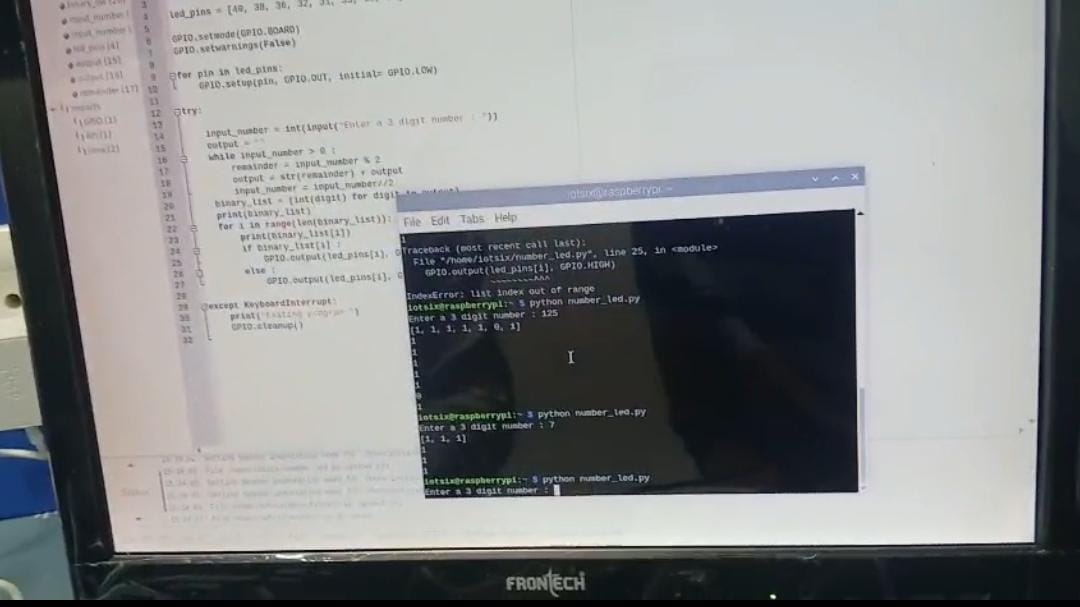
\includegraphics[width=0.62\textwidth, trim=398 102 212 192, clip]{figures/rpi_terminal.jpg}
\caption{Two outputs from a single terminal session on the Raspberry Pi.
\textbf{Output 1:} the input $125$ gives the bit pattern \texttt{1111101}, printed as a
list and then one digit per line; zero-padded to eight places this is
\texttt{01111101}. \textbf{Output 2:} the input $7$ gives \texttt{111}, i.e.\
\texttt{00000111}. The traceback visible at the top is discussed in
Section~\ref{sec:discussion}.}
\label{fig:out1}
\end{figure}

\subsection*{The display itself}

\vspace{2pt}
\noindent
\begin{minipage}[t]{0.485\textwidth}
\centering
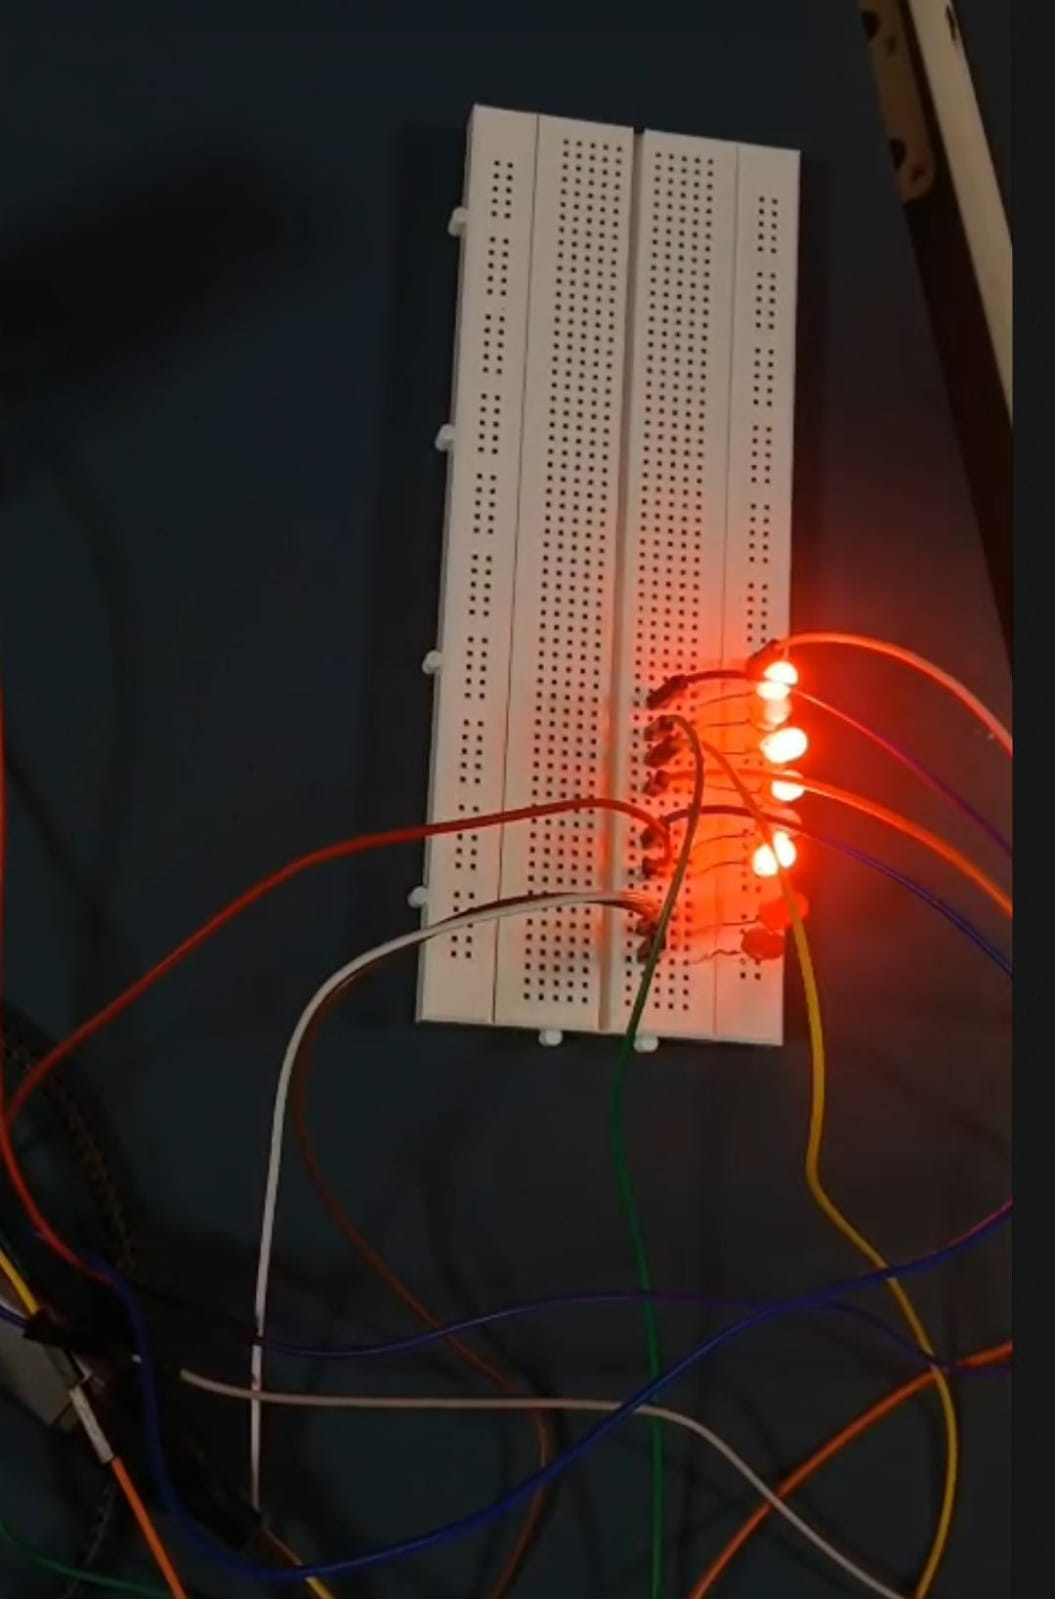
\includegraphics[width=\linewidth, trim=520 519 55 580, clip]{figures/binary_pattern_a.jpg}
\end{minipage}\hfill
\begin{minipage}[t]{0.485\textwidth}
\centering
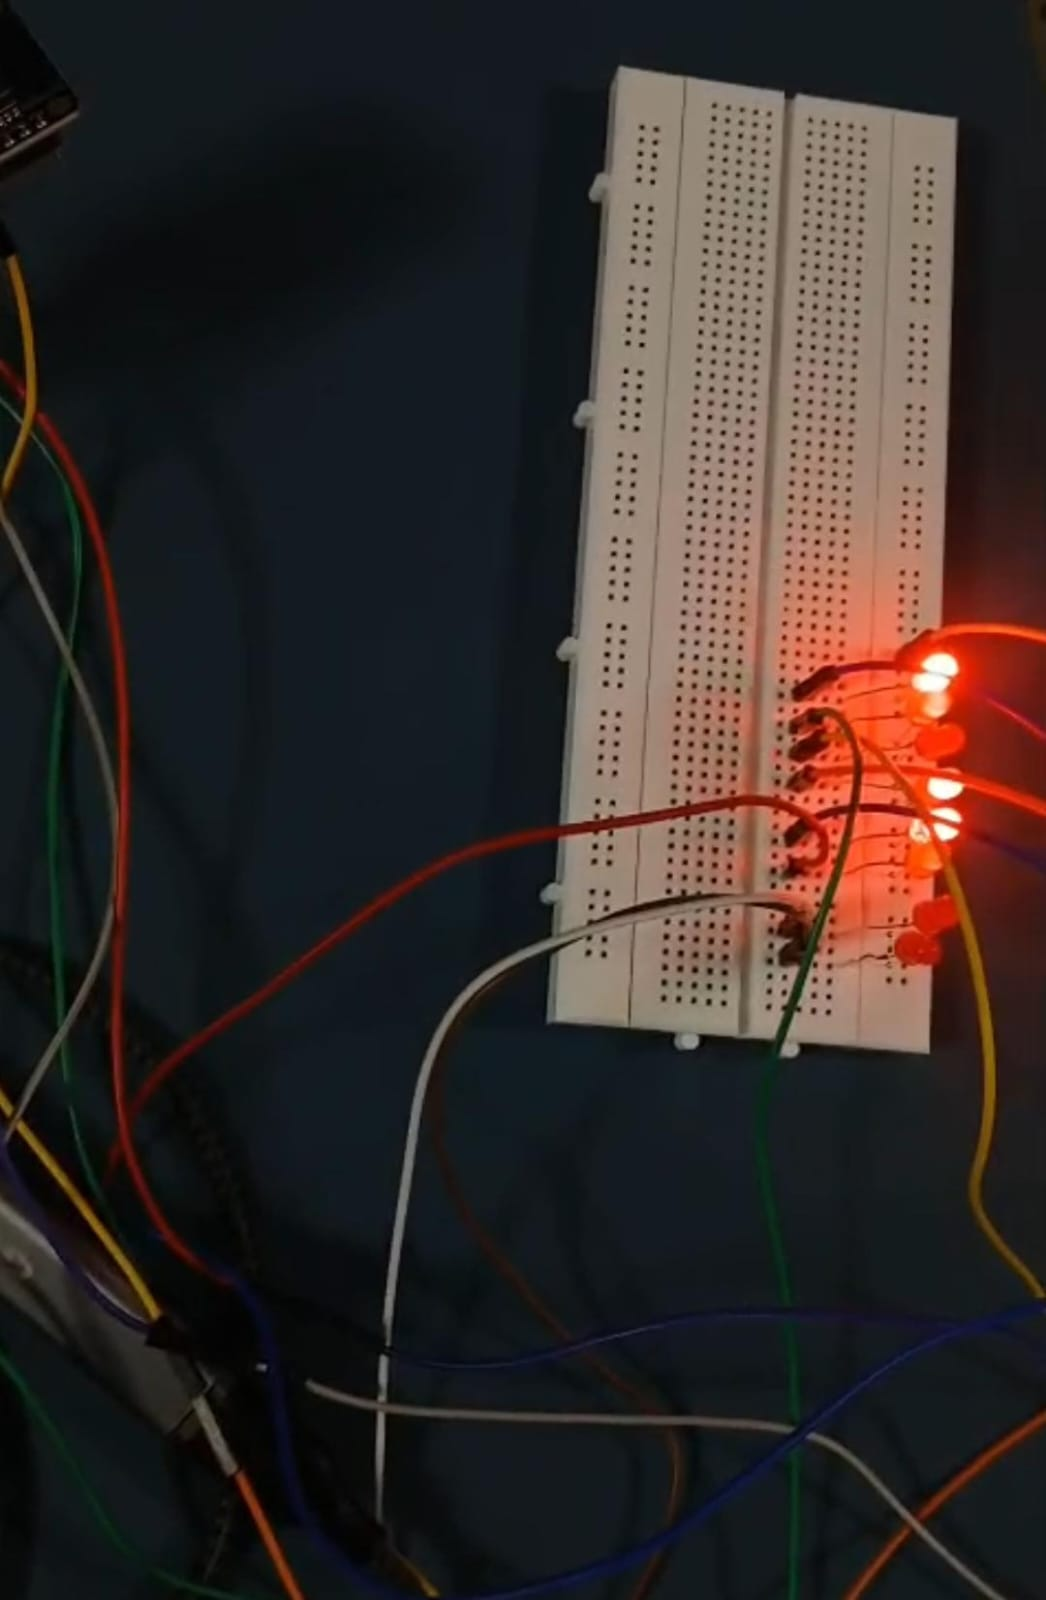
\includegraphics[width=\linewidth, trim=580 540 0 560, clip]{figures/binary_pattern_b.jpg}
\end{minipage}
\captionof{figure}{Two different values displayed on the eight-LED array. The lit LEDs
correspond to the set bits of the number entered on the console; changing the input
changes the pattern immediately.}
\label{fig:patterns}

\vspace{10pt}

\begin{figure}[H]
\centering
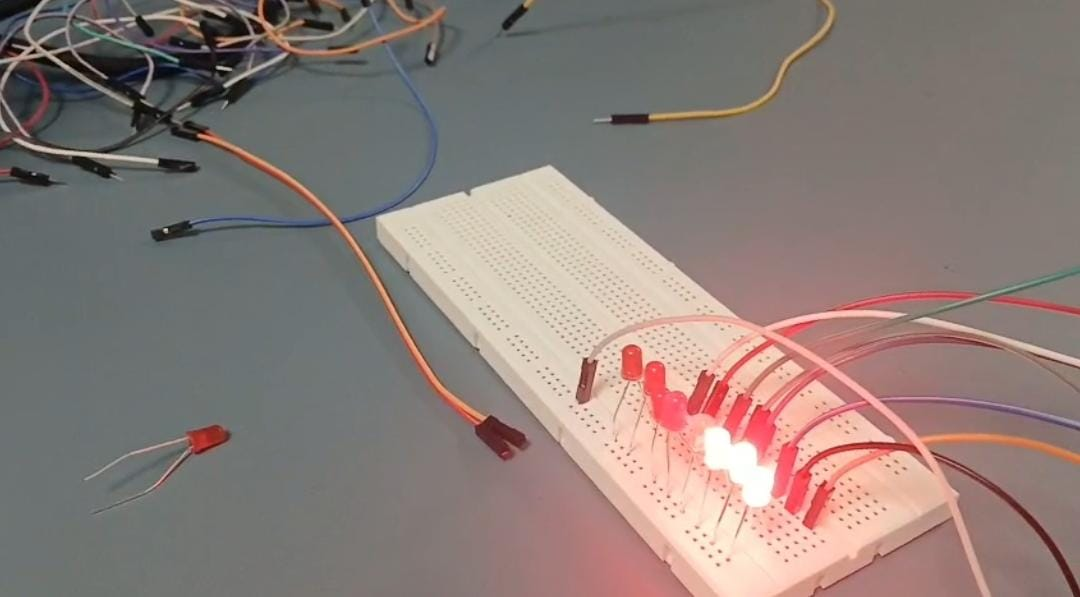
\includegraphics[width=0.62\textwidth]{figures/rpi_8led_setup.jpg}
\caption{The assembled circuit --- eight LEDs in a row on the breadboard, each wired
directly to its own GPIO pin, with the cathodes on the common ground rail.}
\label{fig:setup}
\end{figure}

\subsection*{Video demonstration and code}

\begin{titledbox}[before skip=6pt]{Google Drive link}
\noindent The demonstration videos, this report and the complete source code are
available in the following shared folder:

\vspace{4pt}
\noindent\drivefolder

\vspace{4pt}
{\small\color{cmnt} Access has been set to \emph{anyone with the link can view}.}
\end{titledbox}

\subsection*{Discussion}
\label{sec:discussion}
\begin{itemize}
  \item The bit string \emph{must} be zero-padded to eight digits. An earlier version of
        the program built the bit list by repeated division, which yields only as many
        digits as the number needs --- seven for $125$ and only three for $7$, both
        visible in Figure~\ref{fig:out1} --- and indexing eight pins against that shorter list
        raised an \texttt{IndexError: list index out of range}. Using
        \texttt{format(number, '08b')} fixes this by always producing exactly eight
        characters.
  \item Wiring the most significant bit first means the row of LEDs can be read
        left-to-right in the same order as the printed binary string, which made
        checking each output against the console immediate.
  \item Because no series resistors were used, the LEDs were driven close to the pin's
        current limit. This is acceptable for a short demonstration, but a
        $220\,\Omega$ resistor per LED would be the safer arrangement, particularly
        here where up to eight pins can source current at once.
  \item Input validation matters: a value above $255$ cannot be represented in eight
        bits and would silently lose its high bits, so the program rejects anything
        outside the range rather than displaying a wrong pattern.
\end{itemize}

%------------------------------------------------------------------ CONCLUSION
\section{Conclusion}

The experiment demonstrated how a group of GPIO pins can be treated together as a
\textbf{parallel output port} rather than as independent switches. Eight LEDs driven
from eight pins of a Raspberry Pi were used to display any decimal number from $0$ to
$255$ as its 8-bit binary equivalent, with the pattern of lit LEDs matching the binary
string computed in software for every value tested.

The exercise linked a software representation directly to a physical one: converting a
number to binary, mapping each bit to a pin, and reading the result back off the
hardware. The pattern of lit LEDs agreed with the binary string printed on the console
for every input tested, confirming that the conversion and the wiring were both
correct.

\end{document}
